\chapter{Card-Sorting}
\label{chap:Card-Sorting}

In general, card sorting is a technique in user experience. Participants 
of a study have to assign the different cards into the matching 
category, which is more or less a low-tech approach. 

It is mostly used for designing a navigation structure, but it can be used 
for evaluating an information architecture of a website or any other 
information structure, too.
A sample image of card sorting can be viewed in Figure~\ref{fig:sample}. 

\begin{figure}[tp]  \centering
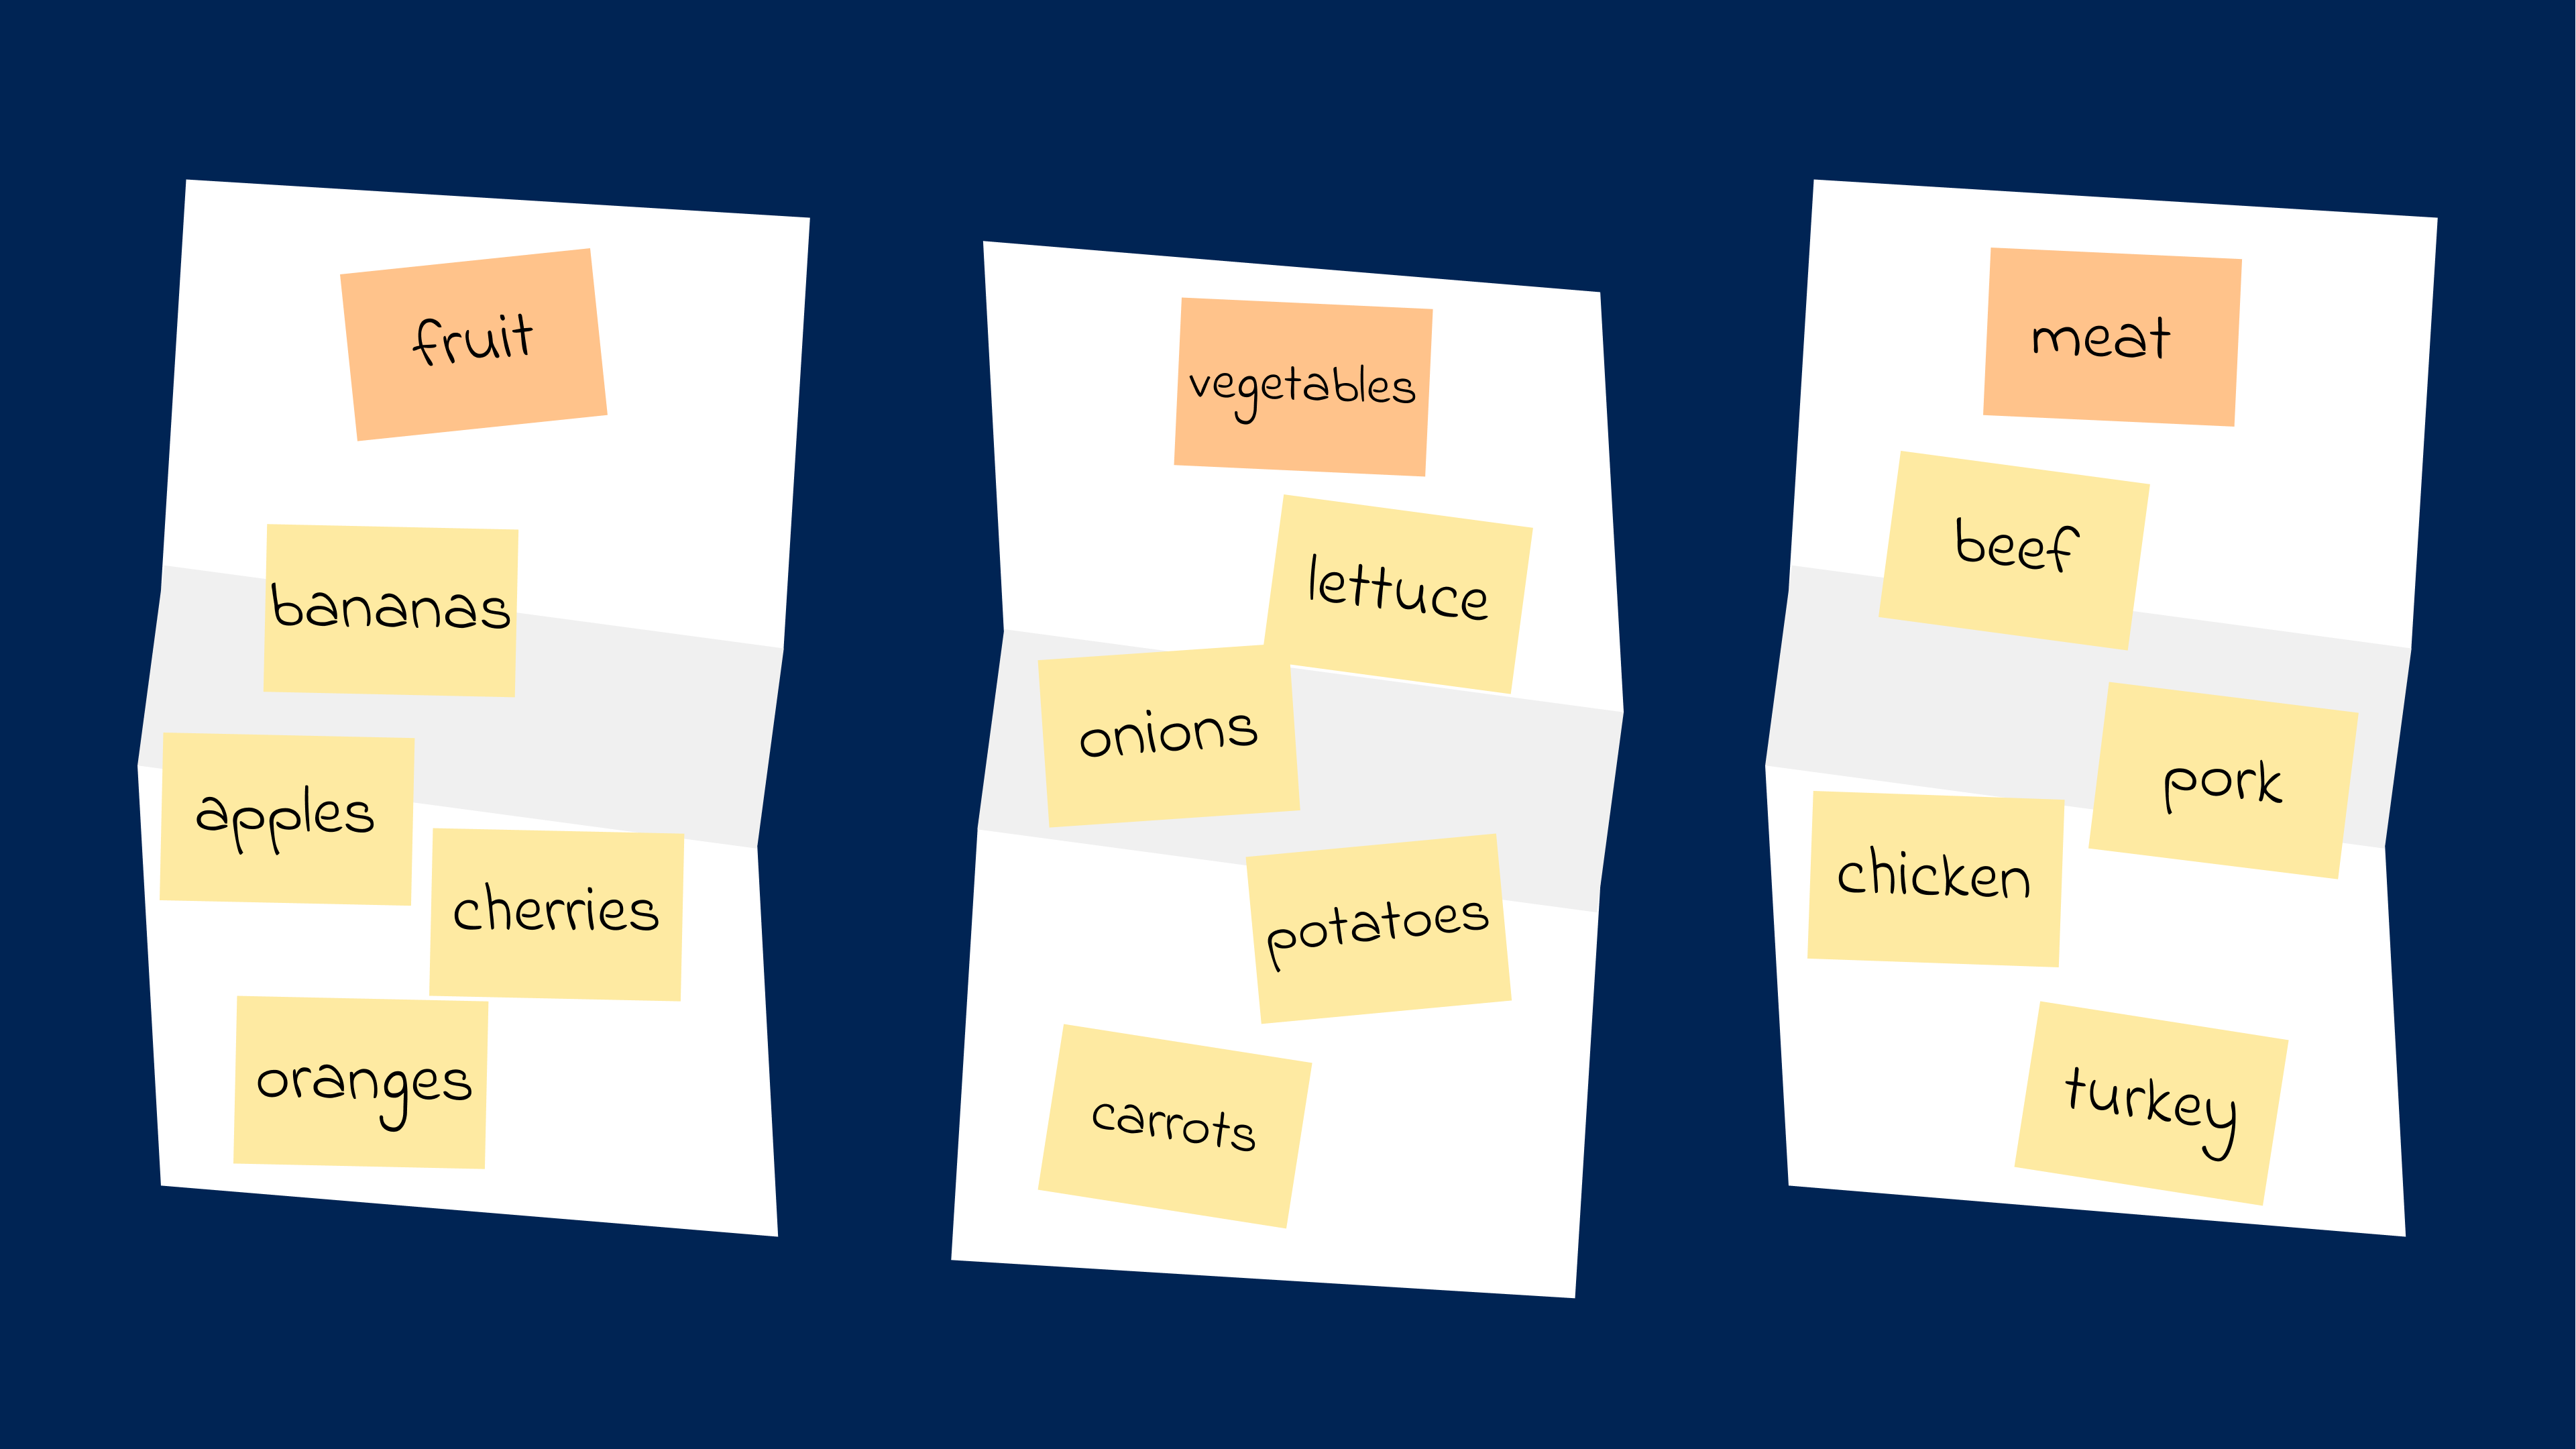
\includegraphics[keepaspectratio,width=\linewidth,height=\halfh]{images/card-sorting/sample.png}
\caption[Sample Image of Card Sorting] 
{A sample image of a card sorting shows dividing cards in three categories.
\imgcredit{Drawn by Markus Stradner, inspired by the illustrations accompanying Sara Jee Watson's blog post  (\url{https://boagworld.com/usability/card-sorting/)}.} } 
\label{fig:sample} 
\end{figure}


\section{Procedure}
All in all, participants of a card sorting study simply assign cards to the 
respective categories, which they believe makes sens. The exact procedure 
depends on the defined variant. 


\section{Variants}
There are three different types of card sorting. At the closed card sorting 
the users have a fixed setup for the categories and at the open card sorting 
they have to create the different categories for their own. But there is also 
a hybrid variant where you actually have a closed card sorting but you are 
also be allowed to add new categories.  






